\chapter{等额年金}
\section{符号一览}
\noindent$a_{\angles{n}},s_{\angles{n}}$\\	$\ddot{a}_{\angles{n}}$\\$\ddot{s}_{\angles{n}}$
\section{等额年金}
\begin{definition}{年金的终值与现值}
\noindent $a_{\angles{n}},s_{\angles{n}}$\\
$s_{\angles{n}}=a_{\angles{n}}(1+i)^{n}=\frac{(1+i)^{n}-1}{i}$
\end{definition}
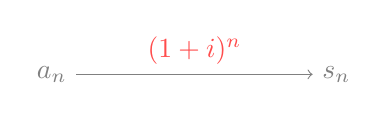
\begin{tikzpicture}
\draw [color=black!50,->](0,0) node[left]{$a_{\angles{n}}$}-- node [color=red!70,pos=0.5,above,sloped]{$(1+i)^n$}(3,0) node[right]{$s_{\angles{n}}$};
    \end{tikzpicture} \\
\noindent $a_{\angles{n}}=v+v^2+v^3+\dots+v^n=\frac{1-v^n}{i}=\frac{1-\frac{1}{(1+i)^n}}{i}=\frac{1-v^n}{\frac{1}{v}-1}$\\
$\ddot{a}_{\angles{n}}=\frac{1-v^n}{d}$ \\
$s_{\angles{n}}=a_{\angles{n}}(1+i)^{n}=\frac{(1+i)^{n}-1}{i}$\\
$\ddot{s}_{\angles{n}}=\ddot{a}_{\angles{n}}(1+i)^{n}=\frac{(1+i)^{n}-1}{d}$
